
\section{Infrastruktūras pārvaldība}
\label{sec:ops}

Attēlā \ref{fig:hwstream} redzama demo laboratorija, kas uzstādīta darba autora
mājās, Kalnciema ielā. Lai gan nodaļā \ref{sec:dipplatform} redzamā 0. līmeņa
DPD diagramma, šķietami, gana ilustrē platformas konceptuālo uzbūvi, iespējams
ir vērtīgi aplūkot fiziskā līmenī izmantoto publisko testa platformu
\cite{VeinbahsKrisjanisProduction}. Attēlā \ref{fig:production} redzama šāda
testa platformas fiziskā līmeņa arhitektūra. Testa platformas serveris tika
uzstādīts DigitalOcean mākoņpakalpojumu devēja virtuālmašīnā, kas atrodas datu
centrā Frankfurtē jeb Vācijā. Savukārt, pati laboratorija ar platformas aģentu
un \glslink{board}{aparatūru} atradās Kalnciema ielā jeb Latvijā. Arī
\glslink{firmware}{programmaparatūras} izstrādātājs jeb darba autors, atradās
Latvijā kafejnīcā ar bezvada tīklu.

\begin{figure}[H]
    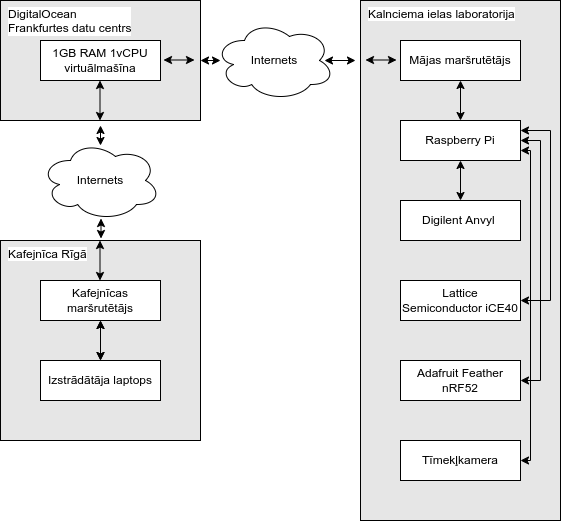
\includegraphics[width=0.8\linewidth]{assets/production.drawio.png}
    \centering
    \caption{Platformas testa vides fiziskā līmeņa arhitektūra.}
    \label{fig:production}
\end{figure}

Veicot attālinātu \glslink{firmware}{programmaparatūras} izstrādi datu plūsma
notika starp šo fizisko iekārtu tīklu. Tieši šajā arhitektūrā arī lielākoties
notika platformas izstrāde un testēšana tai skaitā demo
\glslink{firmware}{programmaparatūras} izstrāde un testēšana. Darba izstrādes
laikā tīkla latence starp šīm iekārtām nebija būtiski jūtama un būtiski
neietekmēja darba izstrādi.

Papildus jāmin, ka attēlā \ref{fig:production} redzama vairāk fiziska
\glslink{board}{aparatūra} nekā aprakstīta šajā darbā, taču oriģināli
prototipējot darba arhitektūru, tika secināts, ka arī šādas ierīces ir iespējams
pievienot platformai, taču laika ierobežojumu dēļ tām netika izstrādāts atbalsts
platformas komandu rindas aģenta rīkā. 

\section{Platformas programmaparatūras minimālās prasības}
\label{sec:minrequirements}

Lai izmantotu izstrādāto platformu, ir jābūt piekļuvei centralizētam
\glslink{server}{serverim}, piemēram, darba autora publiski uzstādītajam testa
serverim. Lai mijiedarbotos ar platformu, ir nepieciešami komandu rindas rīki,
kas nedara neko vairāk par savienojuma izveidi, datu apmaiņu un virtuālās
\glslink{vinterface}{saskarnes} gadījumā krāsainu simbolu attēlošanu komandu
rindā.

Šo servera programmatūru un komandu rindas rīku programmatūru, visticamāk, spēj
izpildīt lielākā daļa datoru, kas iegādāti pēdējos 10 gados.  Taču, lai
mijiedarbotos ar \glslink{board}{FPGA attīstītājrīku aparatūru}, ir nepieciešama
gana spējīga aparatūra, kas nav triviāls jautājums. \gls{fpga} aparatūra
mūsdienās joprojām ir ļoti ierobežota tai pieejamo \gls{lcs} skaitā, tādēļ ir
būtiski pārliecināties, iegādājoties jaunu \gls{fpga} aparatūru, ka tai ir gana
daudz \gls{lcs} elementu, lai darbinātu platformas programmaparatūru. Tādēļ
tabulā \ref{table:lcusage} ir aprakstīts \gls{lcs} jeb loģisko elementu un IO
jeb ievades un izvades signālu patēriņš atkarībā no platformas programmatūras un
tās konfigurācijas.

\begin{table}[H]
    \begin{tabular}{ |p{5cm}|p{3cm}|p{3cm}| }
    \hline
        & A & B\\
    \hline
    Ir 8xLED displejs & Jā & Jā \\
    Ir 8x slēdži & Jā & Jā \\
    Ir 24x spiedpogas & Jā & Jā \\
    Ir 64x RGB LED displejs & Jā & Nē \\
    Ir 32x baitu teksta izsūtne & Jā & Nē \\
    Ir 32x baitu teksta iesūtne & Jā & Nē \\
    \hline
    IOs & 11 & 3 \\
    LCs & 5932 & 773 \\
    \hline
    Ietilpst Spartan-6 & Jā & Jā \\
    Ietilpst ICE40-HX1K & Nē & Jā \\
    \hline
    \end{tabular}
    \centering
    \captionsetup{justification=centering}
    \caption{Programmaparatūras \gls{lcs} patēriņš atkarībā no konfigurācijas}
    \label{table:lcusage}
\end{table}

Tabulā \ref{table:lcusage} pieminētā A konfigurācija ir sākotnēji izstrādātā,
iepriekš aprakstītā, MinOS virtuālās saskarnes programmaparatūra ar visiem
realizētajiem mijiedarbības un grafiskajiem elementiem, kas tika izmantota
Spartan-6 \gls{fpga}.

Darba izstrādes laikā eksperimentējot, tika testēta programmaparatūras
augšupielāde mazāk spējīgajā ICE40-HX1K \gls{fpga} un tika secināts, ka tā kā
tam ir tikai 1280 \gls{lcs}, tad tas nav savietojams ar 5932 \gls{lcs} A
konfigurācijas platformas programmaparatūru. Tādēļ no šīs pilnās virtuālās
saskarnes programmaparatūras tika noņemti elementi līdz programmaparatūra
ietilpa šajā \gls{fpga}, tādējādi iegūstot konfigurāciju B. B konfigurācijā
programmaparatūrā ir noņemti monitora un teksta elementi, kā arī 8xLED vērtību
attēlošana uz fiziskās \glslink{board}{aparatūras} LED gaismām (tādējādi
atstājot to attēlošanu tikai virtuālajā saskarnē un ne tīmekļa kameras
saskarnē).  

Šis mazāk spējīgā \gls{fpga} trūkums arī iezīmē digitālo iekārtu projektēšanā
aktuālu problēmu - tranzistoru skaits prototipēšanā nav bezgalīgs, tādēļ ir
jābūt ļoti radošam to ekonomēšanā un tātad projektēšanā. 

Vērts pieminēt, ka tabulā \ref{table:lcusage} redzamie dati tika iegūti
sintezējot \gls{netlist}{Netlist konfigurācijā} platformas MinOS saskarnes
programmaparatūras Verilog \gls{hdl} projektējumu ar \lstinline!yosys! atvērtā
koda rīku, pēc tam to pārkonvertējot \gls{fpga} binārajā formātā ar
\lstinline!arachne-pnr! atvērtā koda rīku. Avota kods šīm konfigurācijām ir
pieejams projekta repozitorijā. \cite{VeinbahsKrisjanisTestbed}

\section{Platformas lietojamība un uzturēšana}
\label{sec:maintenance}

Darba izstrādes laikā tika pacelti apsvērumi par šādas platformas uzturamību un
lietojamību, kas apskatīti un aprakstīti šajā nodaļā. J - jautājums, A -
atbilde.

J. Cik sarežģīti laboratorijas īpašniekam ir pieslēgt savu laboratoriju
platformai?

A. Ir nepieciešama papildus \glslink{board}{aparatūra} laboratorijā, kas
funkcionēs kā komunikācijas starpnieks starp platformu un
\glslink{board}{aparatūru}, jeb ir nepieciešams aģenta dators vai
mikrokontrolieris. Aģentu nepieciešams administrēt, tajā jāuzstāda
\glslink{board}{aparatūras} pārvaldības \glslink{software}, ko parasti nodrošina
\glslink{board}{aparatūras} ražotāji. Aģentā nepieciešams uzstādīt platformas
komandu rindas aģenta rīku. Lai optimizētu šo administrēšanas procesu tehniski
ir iespējams izstrādāt Ansible, Chef vai citu automatizācijas risinājumu
skriptus, lai automātiski nokonfigurētu aģenta sistēmu. Papildus, ja ir aģenti
nepieciešami ir daudz, tehniski Raspberry mikrokontroliera gadījumā ir iespējams
izstrādāt sistēmas attēla kopiju, ko var pārkopēt citā SD kartē, ko var ievietot
nākamajā Raspberry mikrokontrolierī, tādējādi vienkāršojot aģentu uzstādīšanas
procesu. Darba ietvaros šīs divas optimizācijas nav mēģināts izstrādāt laika
ierobežojumu dēļ.

J. Cik sarežģīti platformas autoram ir izstrādāt jaunu platformas versiju?

A. Platformas pirmkoda kompilēšana ir automatizēta. Pirmkoda repozitorijā ir
fails \lstinline!build.sh!, kas automātiski sakompilē platformas
\glslink{server}{servera} Scala pirmkodu ar \lstinline!sbt! rīku, automātiski
sakompilē platformas aģenta un klienta komandu rindas rīkus \lstinline!AMD64! un
\lstinline!ARM64! procesoru arhitektūrām (\lstinline!ARM64! nepieciešams, lai
darbinātu aģentu Raspberry Pi mikrokontrolierī vai Apple datorā ar M1 procesoru)
un ar \lstinline!pip! rīku un \lstinline!docker buildx!, kas atbalsta
multi-platformu kompilāciju, \cite{DockerBuildx}. Lai autora darbs būtu vēl
vieglāks šo visu varētu automatizēt kādā nepārtrauktās integrācijas platformā,
piem. Jenkins, Drone CI, Concourse CI, Hydra CI, u.c..

J. Cik sarežģīti platformas izstrādātājam ir sākt lietot platformu?

A. Lai sāktu izmantot platformā pieejamo \glslink{board}{aparatūru}, ir
izstrādāts skripts, lai automātiski datorā ieinstalētu platformas komandu rindas
klienta rīku. Tekstā \ref{lst:setup} redzams, ka no klienta ieinstalēšanas līdz
\glslink{firmware}{programmaparatūras} augšupielādei un lietošanai ir tikai trīs
komandas, neskaitot lietotāja un tā tiesību izveidošanu, ko tipiski darītu
laboratorijas vai platformas īpašnieks.

Papildus ir vērts pieminēt, ka pieejamā platforma tika atrādīta maģistra
studentiem kursā DatZ3074 un saņēma pozitīvas atsauksmes, ka to būtu iespējams
izmantot, lai piemēram projektētu kādu spēli tranzistoru loģikā vai projektētu
galīgus determinētus automātus, utml., kā arī tika saņemti ieteikumi kā
platforma varētu tikt uzlabota ar jaunu funkcionalitāti nākotnē, piem. lai
abstrahētu vairākas \gls{fpga} attīstītājrīku iekārtas vai lai veiktu
paralelizētu datu apstrādi ar ierīču klasteriem. 

\begin{lstlisting}[caption={Platformas klienta lietošanas uzsākšana},label={lst:setup},captionpos=b]
curl -L https://github.com/kshaa/dip-test[...]install.sh | bash
dip_client session-auth -u <username> -p <password>
dip_client quick-run -f firmware.bit -b ${BOARD_UUID}
\end{lstlisting}

\section{Programmaparatūras testēšana}
\label{sec:testing}

Lai gan platformā iespējams augšupielādēt un attālināti mijiedarboties ar
\glslink{firmware}{programmaparatūru}, tās testēšana nebūt nav triviāla.

Viens variants ir testēt \glslink{firmware}{programmaparatūru} manuāli -
attālināti augšupielādēt to attīstītājrīka \glslink{board}{aparatūrā}, uzsākt
virtuālās \glslink{vinterface}{saskarnes} sesiju, mijiedarboties un secināt vai
\glslink{board}{aparatūra} darbojas kā paredzēts. Šis variants ir pilnīgi
pietiekams maza izmēra projektiem, kuriem nav stingru laika ierobežojumu. Šis
arī ir veids kā tika testēta platformas demo \gls{firmware} un tātad šis
testēšanas veids ir pieejams platformā.

Otrs variants ir pirms \glslink{firmware}{programmaparatūras} augšupielādes
\glslink{board}{aparatūrā}, veikt tās programmatisku simulāciju, ko nodrošina
tādi rīki kā \lstinline!iverilog! vai grafiskā izstrādes vide
\lstinline!Xilinx-ISE!. Šis ir viens no svarīgākajiem izstrādātāja
instrumentiem, kas arī tika izmantots testējot demo
\glslink{firmware}{programmaparatūru} un ir izmantojams platformas ietvaros, lai
gan tehniski ir ārpus-platformas rīks.

Trešais variants ir testēt \glslink{firmware}{programmaparatūras} darbību
programmatiski.Un pat šim variantam ir divi veidi - testēt reāllaikā un testēt
post-factum. 

Platformas ietvaros tika izstrādāta virtuālā \glslink{vinterface}{saskarne}
\lstinline!minosrequest!, kas ļauj definēt laikus, kad iesūtīt
\glslink{vinterface}{saskarnē} ziņas, un kas ieraksta visas ienākošās un
izejošās ziņas JSON formātā. Ar šo saskarni ir iespējams realizēt post-factum
darbības testēšanu veicot datu jeb ziņu analīzi jebkurā programmēšanas valodā,
kas spēj parsēt JSON datus. Kā piemēru analizējamiem datiem, var skatīt JSON
ierakstu pielikumā \ref{att:minosrequest}.

Lai testētu \glslink{firmware}{programmaparatūras} darbību reāllaikā ir dažādas
realizācijas iespējas. Viens variants ir skaidri dokumentēt platformas seriālās
komunikācijas WebSocket API un izmantoto protokolu, kas ļautu jebkurā
programmēšanas valodā viegli attālināti pieslēgties \glslink{board}{aparatūrai}
un definēt jebkāda veida mijiedarbību vai papildus virtuālu
\glslink{vinterface}{saskarni}, vai testus, u.t.t. Šī ir laba ideja, kas nav
realizēta darba ietvaros laika ierobežojumu dēļ.

Iepriekšminētajai pieejai gan ir viens mīnuss, kas ir, ka izstrādātājam ir vai
nu jābūt ieslēgtam laptopam vai arī jāuztur sava infrastruktūra, lai veiktu
ilgtermiņa (stundas vai dienas) testus. Potenciāls risinājums šim ir iestrādāt
platformas \glslink{server}{serverī} \gls{wasm} atbalstu un ļaut iesūtīt WASM
programmatūru, kas darbotos platformā, saņemtu ziņas, sūtītu atpakaļ ziņas,
rakstītu žurnāla datus, secinātu vai apratūra darbojas korekti. Šādai pieejai
arī būtu pluss, ka visi izvadītie testa dati būtu standartizēti un pieejami
platformā. Darba ietvaros tika veikti eksperimenti un tika secināts, ka Scala
programmēšanas valodā ir WASM virtuālmašīnas darbināšanas atbalsts, taču laika
ierobežojumu dēļ, ideja netika tālāk izpētīta.
